To study the performance of compressed word embeddings in downstream tasks, we begin by empirically comparing methods with different underlying machineries. In our attempt to understand what intrinsic characteristic determines the downstream performance across different compressed embedding types, we observe that PIP loss and $(\Delta_1, \Delta_2)$-spectral approximation error, as compression quality metrics, can poorly correlate with downstream performance across the simple uniform quantization and state-of-the-art methods. This impose challenges to understand what intrinsic characteristic determines the downstream performance of compressed embeddings in a principle.
In particular, we observe the simple fast uniform quantization approach can compete with state-of-the-art deep compositional code learning (DCCL) \citep{dccl17} and k-means based compression \citep{andrews16} across various NLP tasks at different compression rates. However, the simple quantization method can have significantly worse compression quality metric while matching the downstream performance of the state-of-the-art methods. In this section, we discuss our empirical comparison of compression methods, and demonstrate the lack of correlation between existing metrics and downstream task performance. These observations motivates our new compression quality metric in Section~\ref{sec:new_metric} which correlates well with downstream performance; it leads to a more principled understanding on how compression impacts generalization. 


\subsection{Performance Comparison}
\label{sec:perf_comp}
\todo{(dataset info might be need to be added)} In our empirical performance comparison of the different compression method, we evaluate the embeddings compressed by each method on a variety of tasks. We demonstrate that the compressed embeddings based on simple uniform quantization can match the the state-of-the-art DCCL and k-means method. To compare these methods on different uncompressed embedding types, we consider compressing both 300 dimensional GloVe pre-trained embedding and \todo{bla dim} FastText pretrained embeddings. In the experiment with GloVe uncompress embedding, we also include different dimensional GloVe pre-trained embeddings, and use it to compare the performance of compressing high dimensional embeddings and directly using lower dimensional pre-trained embeddings with the same memory footprint. In Figure~\ref{fig:perf_comp}, we can observe across the four tasks using both GloVe and FastText embeddings, the simple uniform quantization method can closely match the DCCL and k-means approach in downstream performance at high compression rate. For example, using the DrQA model \citep{drqa17} on the Stanford Question Answering Dataset (SQuAD) \citep{squad16}, uniform quantization attains a compression ratio of 32x with an average F1 score only 0.47\% absolute below the uncompressed GloVe embeddings, while the DCCL method of \citet{dccl17} is 0.43\% below. Additionally, we observe in Figure~\ref{fig:perf_comp} (top) that compressing higher dimensional word embeddings can perform significantly better than using lower dimensional pre-trained embeddings with the same memory consumption.

\begin{figure*}
	\centering
	%	\begin{tabular}{c c c c}
	\begin{tabular}{@{\hskip -0.0in}c@{\hskip -0.0in}c@{\hskip -0.0in}c@{\hskip -0.0in}c@{\hskip -0.0in}}
		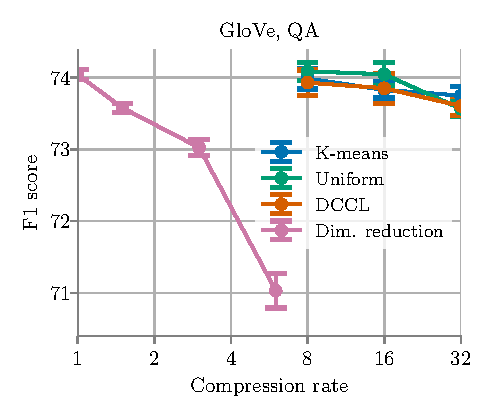
\includegraphics[width=.245\linewidth]{figures/glove400k_qa_best-f1_vs_compression_linx.pdf} &
		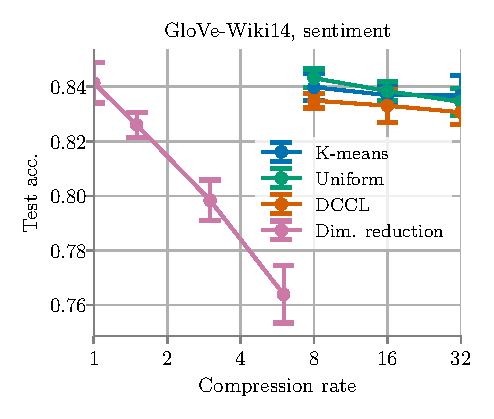
\includegraphics[width=.245\linewidth]{figures/glove400k_sentiment_sst_test-acc_vs_compression_linx.pdf} &
		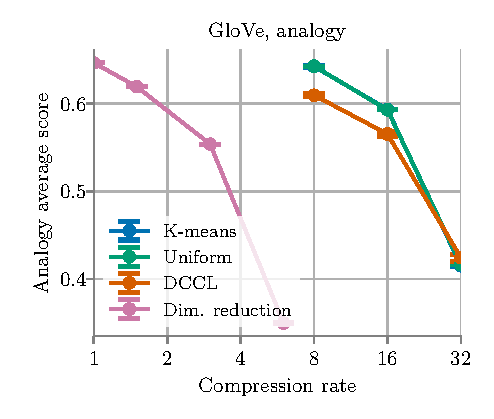
\includegraphics[width=.245\linewidth]{figures/glove400k_intrinsics_analogy-avg-score_vs_compression_linx.pdf} &
		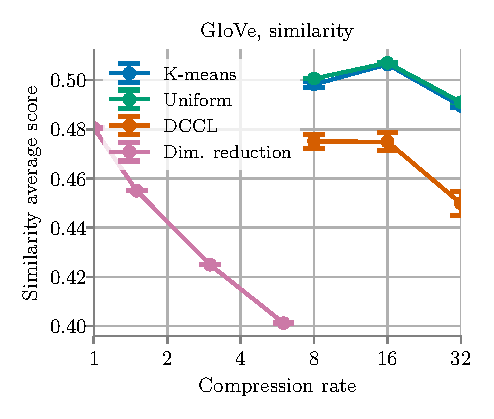
\includegraphics[width=.245\linewidth]{figures/glove400k_intrinsics_similarity-avg-score_vs_compression_linx.pdf} \\
		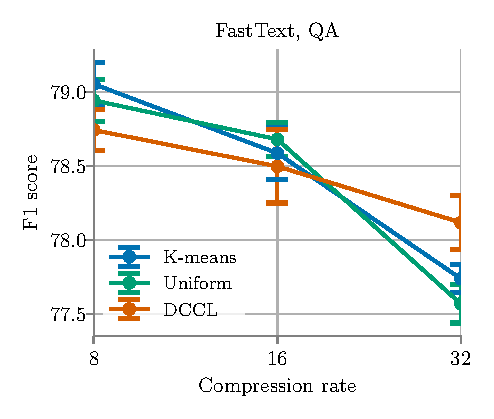
\includegraphics[width=.245\linewidth]{figures/fasttext1m_qa_best-f1_vs_compression_linx.pdf} &
		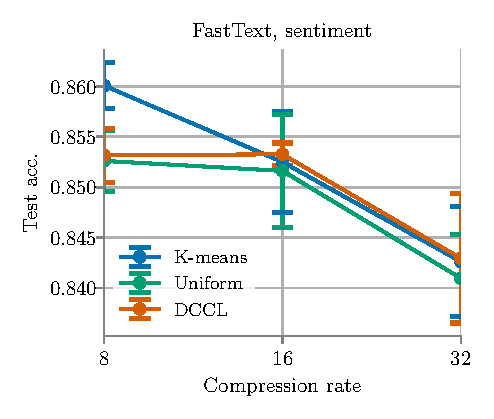
\includegraphics[width=.245\linewidth]{figures/fasttext1m_sentiment_sst_test-acc_vs_compression_linx.pdf} &
		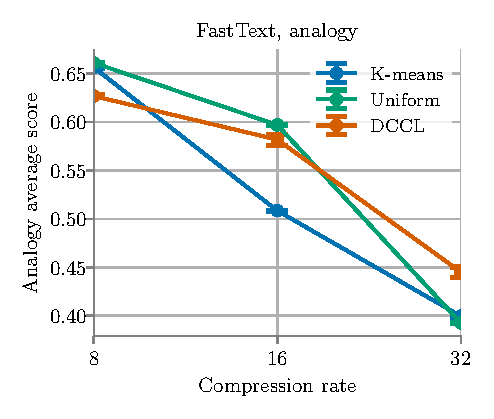
\includegraphics[width=.245\linewidth]{figures/fasttext1m_intrinsics_analogy-avg-score_vs_compression_linx.pdf} &
		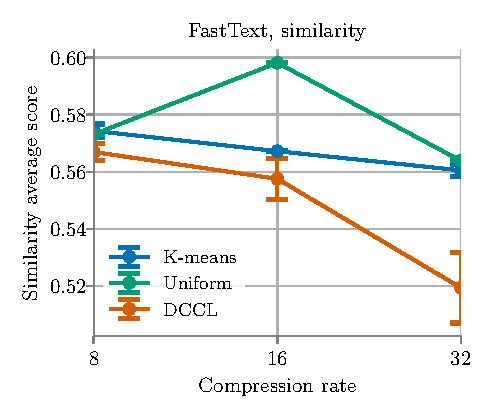
\includegraphics[width=.245\linewidth]{figures/fasttext1m_intrinsics_similarity-avg-score_vs_compression_linx.pdf} \\
		\;\;\;\;\;(a) & \;\;\;\;\;\;(b) & \;\;\;\;\;\;(c) & \;\;\;\;\;\;(d)
	\end{tabular}
\caption{Performance of compressed GloVe (top) and fastText (bottom) embeddings on question answering (a), sentiment analysis (TREC dataset) (b), word analogy (c), and word similarity (d) tasks.
Uniform quantization performs similarly to k-means and DCCL on question answering and sentiment analysis;
on the word analogy and similarity tasks, uniform quantization once again performs similarly to k-means, but outperforms the DCCL method.
For the GloVe experiments, we are also able to compare with pre-trained embeddings of smaller dimensions ($d\in\{50,100,200,300\}$), and observe that compressing the 300-dimensional embeddings is significantly better than using lower-dimensional full-precision embeddings (``Dim. reduction'').
}
	\label{fig:perf_comp}
\end{figure*}


\begin{figure*}
\centering
	\begin{tabular}{@{\hskip -0.0in}c@{\hskip -0.0in}c@{\hskip -0.0in}c@{\hskip -0.0in}c@{\hskip -0.0in}}
		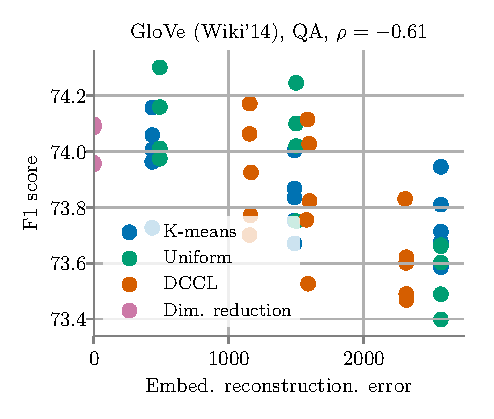
\includegraphics[width=.245\linewidth]{figures/glove400k_qa_best-f1_vs_embed-frob-error_linx.pdf} &
		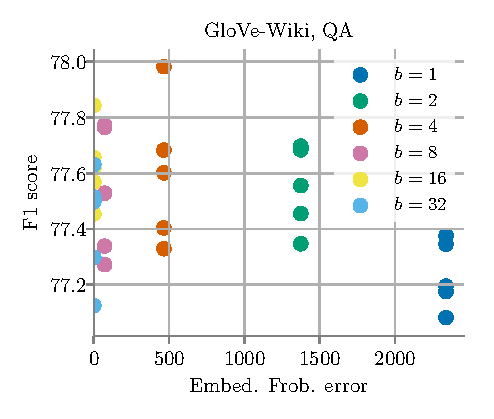
\includegraphics[width=.245\linewidth]{figures/glove-wiki400k-am_qa_best-f1_vs_embed-frob-error_linx.pdf} &
		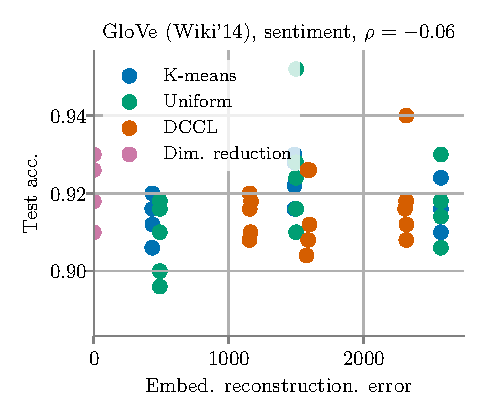
\includegraphics[width=.245\linewidth]{figures/glove400k_sentiment_trec_test-acc_vs_embed-frob-error_linx.pdf} &
		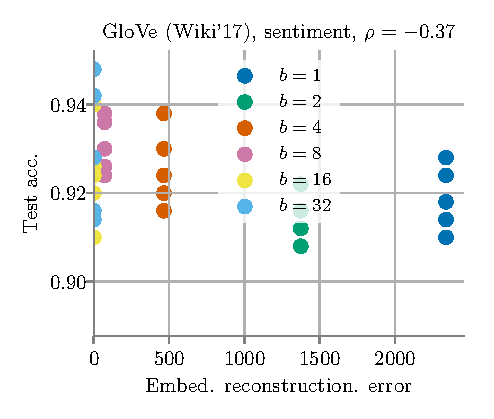
\includegraphics[width=.245\linewidth]{figures/glove-wiki400k-am_sentiment_trec_test-acc_vs_embed-frob-error_linx.pdf} \\
		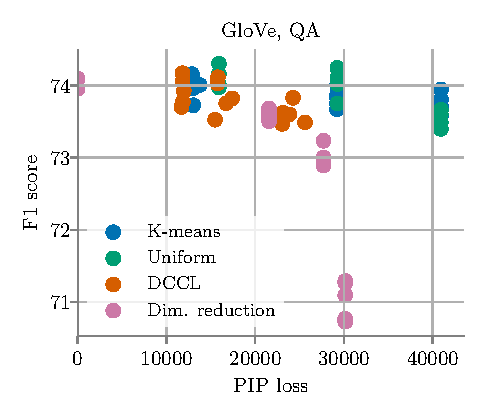
\includegraphics[width=.245\linewidth]{figures/glove400k_qa_best-f1_vs_gram-large-dim-frob-error_linx.pdf} &
		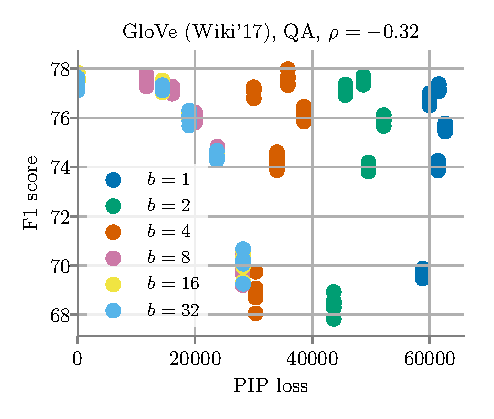
\includegraphics[width=.245\linewidth]{figures/glove-wiki400k-am_qa_best-f1_vs_gram-large-dim-frob-error_linx.pdf} &
		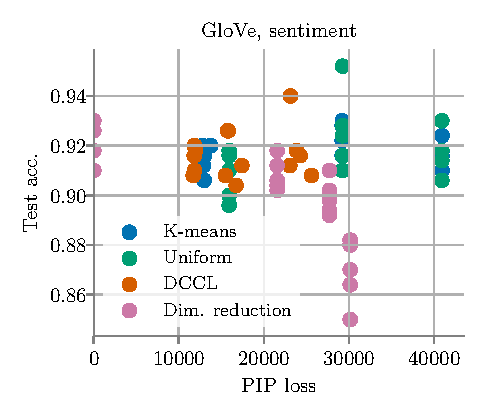
\includegraphics[width=.245\linewidth]{figures/glove400k_sentiment_trec_test-acc_vs_gram-large-dim-frob-error_linx.pdf} &
		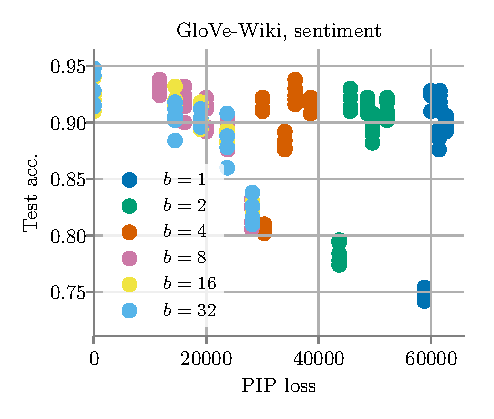
\includegraphics[width=.245\linewidth]{figures/glove-wiki400k-am_sentiment_trec_test-acc_vs_gram-large-dim-frob-error_linx.pdf} \\
		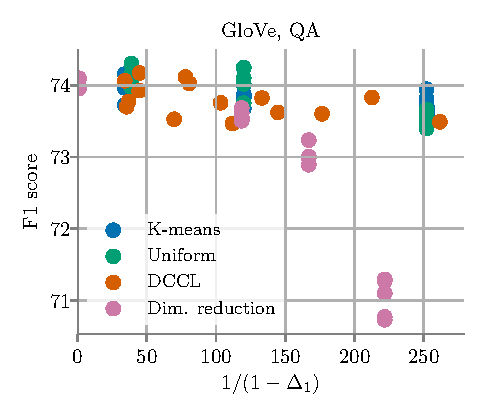
\includegraphics[width=.245\linewidth]{figures/glove400k_qa_best-f1_vs_gram-large-dim-delta1-2-trans_linx.pdf} &
		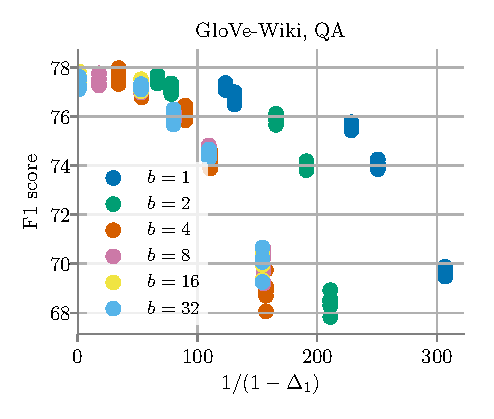
\includegraphics[width=.245\linewidth]{figures/glove-wiki400k-am_qa_best-f1_vs_gram-large-dim-delta1-2-trans_linx.pdf} &
		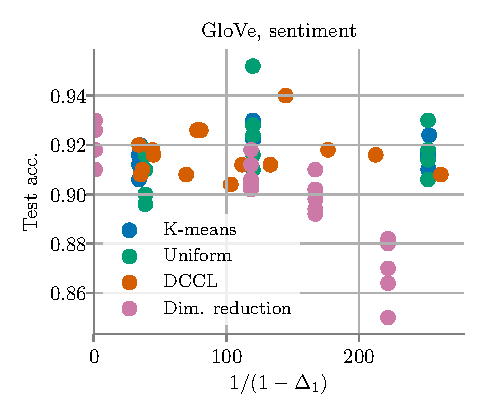
\includegraphics[width=.245\linewidth]{figures/glove400k_sentiment_trec_test-acc_vs_gram-large-dim-delta1-2-trans_linx.pdf} &
		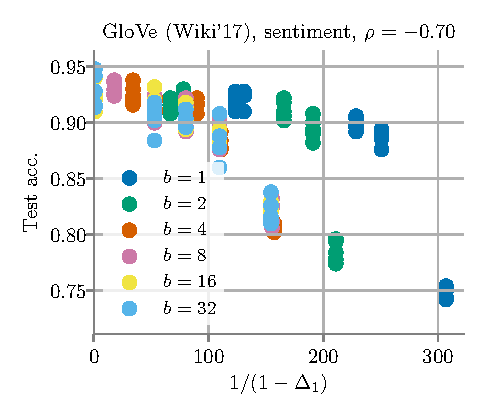
\includegraphics[width=.245\linewidth]{figures/glove-wiki400k-am_sentiment_trec_test-acc_vs_gram-large-dim-delta1-2-trans_linx.pdf} \\
		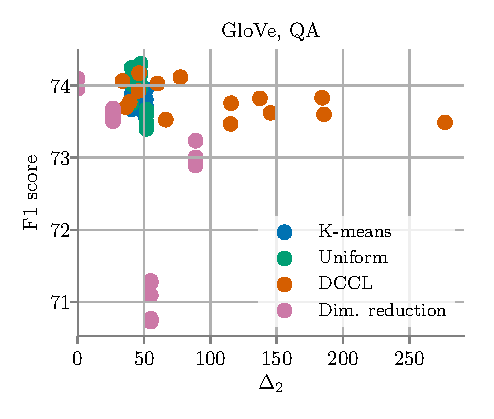
\includegraphics[width=.245\linewidth]{figures/glove400k_qa_best-f1_vs_gram-large-dim-delta2-2_linx.pdf} &
		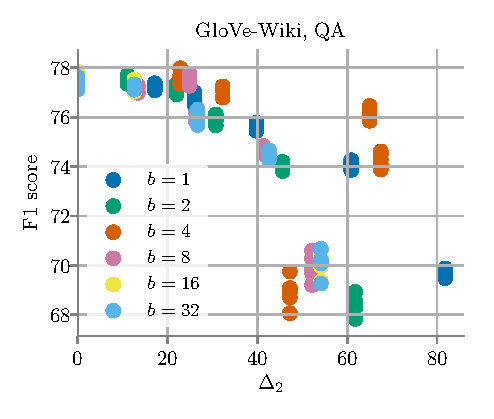
\includegraphics[width=.245\linewidth]{figures/glove-wiki400k-am_qa_best-f1_vs_gram-large-dim-delta2-2_linx.pdf} &
		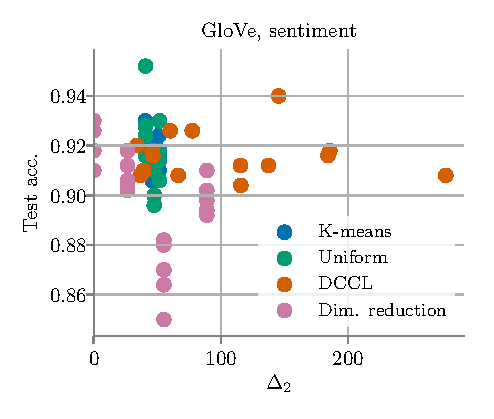
\includegraphics[width=.245\linewidth]{figures/glove400k_sentiment_trec_test-acc_vs_gram-large-dim-delta2-2_linx.pdf} &
		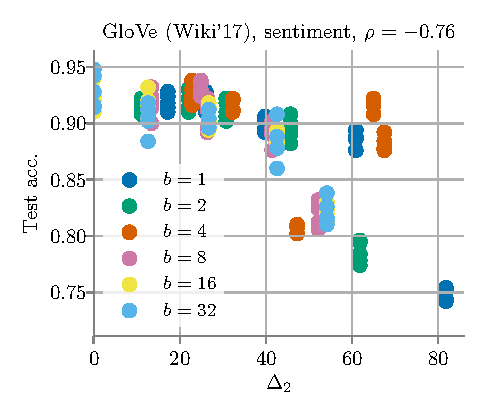
\includegraphics[width=.245\linewidth]{figures/glove-wiki400k-am_sentiment_trec_test-acc_vs_gram-large-dim-delta2-2_linx.pdf} \\
		(a) GloVe, QA & (b) GloVe Wiki, QA  & (c) GloVe, sentiment & (d) GloVe Wiki, sentiment
	\end{tabular}
	\caption{Existing compression quality metric PIP loss and $(\Delta_1, \Delta_2)$-spectral approximation error poorly correlate with the downstream task performance of compressed embeddings. \todo{explain what does adaptive-det mean?} On both the question answering and sentiment analysis task, we demonstrate the PIP loss, $\Delta_1$ and $\Delta_2$ value across different compression method (shown in (a)(c)) and across different precision for the uniform quantization methods (shown in (b)(d)). We can observe in both settings, for example, higher dimensional 1-bit uniform quantization can perform better than lower dimensional uncompressed embeddings (``Dim. reduction''). As another example, uniformly quantized embeddings with different precision can results in similar downstream performance while the compression quality metrics are drastically different.}
	\label{fig:bad_correlation}
\end{figure*}


\subsection{Hardness in Explaining Generalization}
\label{subsec:hard_explain}
To understand why simple uniform quantization can perform as well as state-of-the-art in downstream tasks, we ask the question what intrinsic property of a compressed embedding determines its downstream performance. In particular, we analyze the correlation between existing compression quality metrics and the downstream performance. However, we observe that the metrics we considered in our experiments correlates poorly with the performance of downstream.
Specifically, we consider the Pointwise Inner Product (PIP) loss and the $(\Delta_1, \Delta_2)$-spectral approximation error. This is because many embedding generation methods are implicit matrix decomposition; these two metrics are previously used to understand questions regarding generalization performance for matrix decomposition based supervised learning models \citep{avron17,yin18,lprff18}. 

In Figure~\ref{fig:bad_correlation}, we demonstrate the correlation between downstream task performance and quality metric PIP loss, $\Delta_1$, $\Delta_2$ on both the question answering and sentiment analysis tasks. In Figure~\ref{fig:bad_correlation} (a)(c) we can observe the metrics does not correlate well with generalization performance across different type of compressed embeddings. In this setting, we compress GloVe embeddings with vocabulary size 71,290 on \todo{could you double check here?} and we use the 300 dimensional embedding as the reference embedding to compute the quality metrics. Particularly on both question answering and sentiment analysis, DCCL method and uniform quantization can demonstrate similar generalization performance, but up to 2x different compression quality metrics on both question answering and sentiment analysis. Strikingly higher dimensional 1-bit embeddings outperforms lower dimensional uncompressed embeddings at the same memory footprint with large margin but demonstrate significantly larger PIP loss and $\Delta_2$ values. Furthermore, we also demonstrate the correlation for uniformly quantized embeddings across different quantization precisions, where we compress GloVe with a vocabulary size of 3.8 million and use the 400 dimensional embedding to compute compression quality metrics \todo{could you double check here?}. In Figure \ref{fig:bad_correlation}(a)(c), though 1-bit quantized embeddings show significantly worse compression quality metric than 16-bit quantized embeddings, they can demonstrate similar performance on the downstream tasks. 

An intrinsic characteristic which correlates well with downstream performance is critical to quantitatively understand the generalization of compressed embeddings. However the existing compression quality metrics fail to play this critical role due to poor correlations, which makes understanding the generalization performance challenging without an anchor characteristic. To overcome this problem, we propose a new metric in Section~\ref{sec:new_metric} which correlates well with downstream performance. In the context of linear regression, we prove a generalization bound in terms of this metric for compressed embeddings in Section~\ref{sec:new_metric}. Leverage these understanding built on the new metric, we can then explain why simple uniformly quantized embeddings performs well in a range of downstream tasks with high compression rate.

 
%%%%%%%%%%% info on these embeddings %%%%%%%%%%%%%%%%%%%%%%%%%%%%
%We generate embeddings on two corpora: Text8 with 17 million tokens (vocab size of 71,290) and Wiki with 4.5 billion tokens (vocab size of 3.8 million). The Text8 dataset is the first 100MB of a 2006 cleaned-up dump of Wikipedia where all words are lowercase, numbers are spelled out, and any non-English characters are replaced by whitespace. This data is public available online\footnote{http://mattmahoney.net/dc/text8.zip}. The Wiki dataset is the full English Wikimedia dump on Dec. 4, 2017 which was pre-processed by a fastText script~\footnote{https://github.com/facebookresearch/fastText/blob/master/get-wikimedia.sh} while keeping the letter cases and digits.



%	\begin{itemize}
%		\item Results and claim 1: uniform quantization method can compete well with the state-of-the-art, and it can match uncompressed embedding with high compression rate.
%		\begin{itemize}
%			\item show the generalization performance for quantized embedding and other baselines at different bit rate. (DCCL, kmeans, dimension reduction and uniform quantization)
%			\item Figures on 4 tasks: DrQa, one sentiment, one word analogy and one word similarity
%			\item Tables on tasks performance and time
%		\end{itemize}
%		\item Results and claim 2: Existing matrix reconstruction errors (PIP, spectral approximation error--delta1, delta2) do not correlate well with the generalization performance of compressed embeddings.
%		\begin{itemize}
%			\item Show correlation between performance and Frob norm (PIP) / Deltas (maybe the combination of delta1 and delta2) across a few tasks.
%			\item We can optionally do R2 measurements reliably
%		\end{itemize}
%	\end{itemize}

%\subsection{Preliminary: Embedding Compression Methods}
%\label{subsec:prel}
%%\paragraph{Word Embedding Compression Methods.} 
%\todo{(we should pull prelim as a separate paragraph)}To deploy word embedding to memory constraint settings in data center and edge devices, many methods has been proposed to compress the word embedding. \todo{(we should consider whether we can say kmeans is stoa.)}. Among these methods, state-of-the-art \emph{DCCL approach} \citep{dccl17}\footnote{This idea is also independently adopted by \citet{kway18}.} adopts dictionary learning to represent a large number of word vectors with fewer basis vectors. These basis vectors are organized into multiple dictionaries, and each word is represented as a hash code to discretely combine basis from the dictionaries. In particular, the discrete combination hash code is attained by training an autoencoder with Gumbel-softmax reparameterization \citep{maddison2016concrete,jang2016categorical} to minimize the embedding vector reconstruction error. 
%
%Built on a significantly different machinery, embeddings compressed by a \emph{k-mean method} also demonstrates strong empirical performance in downstream tasks \citep{andrews16}. This k-means method assigns embedding matrix entry values into clusters, and each embedding entries is the approximated by the corresponding cluster center. In this way, one can achieve compression by only storing the cluster id instead of the original value for each embedding matrix entry. 
%
%In contrast to the DCCL and k-mean approach, \emph{uniform quantization} is a simple method requiring no computationally expensive training. This method, as shown in at a high-level in Algorithm~\ref{alg:smallfry}, first clips the embedding matrix into the range $[-r,r]$, and then uniformly quantizes the entries of the clipped matrix; we choose the value of $r$ which minimizes the reconstruction error of the quantized matrix.
%Because our algorithm uses uniform quantization, we first review uniform quantization, and then describe in more detail how our algorithm uses it to compress word embeddings.
%
%
%%\begin{itemize}
%%	\item Briefly describe DCCL and k-means approach
%%	\item Present uniform quantization with Pseudo-code
%%\end{itemize}
%%At a high-level, our algorithm clips the embedding matrix into the range $[-r,r]$, and then uniformly quantizes the entries of the clipped matrix;
%%we choose the value of $r$ which minimizes the reconstruction error of the quantized matrix.
%%Because our algorithm uses uniform quantization, we first review uniform quantization, and then describe in more detail how our algorithm uses it to compress word embeddings.
%
%A \textit{$b$-bit uniform quantization} $Q_{b,r}(x)$ of a real number $x \in [-r,r]$ is computed as follows:
%First, the interval $[-r,r]$ is divided into $2^b - 1$ sub-intervals of equal size.
%Then, $x$ is rounded to either the top or bottom of the sub-interval $[\ulx,\olx]$ containing $x$, where $\ulx = r + j\frac{2r}{2^b-1}$ and $\olx = r + (j+1)\frac{2r}{2^b-1}$, for $j\in\{0,1,\ldots,2^b-2\}$.
%Given this rounded value, one can simply store the $b$-bit integer $j$ or $j+1$ in place of the real-valued $x$, depending on whether $x$ was rounded to $\ulx$ and $\olx$ respectively.
%In this work, we will consider a deterministic rounding scheme which rounds $x$ to the nearest value, and a stochastic rounding scheme which rounds $x$ up or down in such a way that the expected value is equal to $x$.\footnote{
%	This stochastic scheme rounds $x$ to $\ulx$ with probability $\frac{\olx-x}{\olx-\ulx}$ and to $\olx$ with probability $\frac{x-\ulx}{\olx-\ulx}$.
%}
%In particular, our analysis will focus on the stochastic rounding scheme, while our experiments will include results with both schemes.
%%Note that we can upper bound the variance of these rounding schemes using the fact that a bounded random variable in an interval of length $c$ has variance at most $c^2/4$;
%%using this fact, we can see that the variances of these rounding schemes are at most $\frac{1}{4} \cdot \Big(\frac{2r}{(2^b-1)}\Big)^2 = \frac{4r^2}{(2^b-1)^2}$.
%
%
%We are now ready to present the uniform quantization compression algorithm, which we express in pseudo-code in Algorithm~\ref{alg:smallfry}.
%The input to the algorithm is an embedding matrix $X \in \RR^{n\times d}$, where $n$ is the size of the vocabulary, and $d$ is the dimension of the embeddings.
%We define the function $\clip_r(x) = \max(\min(x,r),-r)$ for any non-negative $r$; when matrices are passed in as inputs to this function, it clips the entries in an element-wise fashion.
%The first step in our algorithm is to find the value of $r \in [0,\max(|X|)]$ which minimizes the reconstruction error of the quantized embeddings after $X$ is clipped to $[-r,r]$.
%More formally, we let $r^* \defeq \argmin_{r \in [0,\max(|X|)} \|Q_{b,r}(\clip_r(X))-X\|_F$.
%We then use this value $r^*$ to clip $X$, and then quantize the clipped embeddings to $b$ bits per entry.
%
%In our experiments, we find $r^*$ to within a specified tolerance $\eps > 0$ using the golden-section search algorithm \citep{golden53}.
%To avoid stochasticity impacting the search process, we always use deterministic rounding in the search for $r^*$, even if we use stochastic quantization in the final quantization.
%%this choice also allows us to more cleanly compare deterministic vs.\ stochastic rounding, since they will always use the same value of $r^*$.
%
%\begin{algorithm}[tb]
%   \caption{Uniform quantization for word embeddings}
%   \label{alg:smallfry}
%\begin{algorithmic}[1]
%	\STATE {\bfseries Input:}  Embedding matrix $X \in \RR^{n \times d}$, quantization function $Q_{b,r}$, clipping function $\clip_r\colon\RR\rightarrow[-r,r]$.
%	\STATE {\bfseries Output:} Quantized embeddings $\hat{X}$.
%	\STATE $r^* \defeq \argmin_{r \in [0,\max(|X|)} \|Q_{b,r}(\clip_r(X))-X\|_F$.
%	%Search for $r^* \in [0,\max(|X|)]$ minimizing $\|Q_{b,r}(\clip_r(X))-X\|_F$.
%	\STATE {\bfseries Return:} $Q_{b,r^*}(\clip_{r^*}(X))$.
%\end{algorithmic}
%\end{algorithm}
%
%
%\subsection{Matrix Approximation Error and Generalization}
%Many main stream word embedding generation problem can be casted matrix decomposition \citep{levy2014neural}. For example, Skip-gram Word2Vec \citep{word2vec13} implicitly factorizes the Pointwise Mutual Information (PMI) matrix while GloVe \citep{glove14} decomposes the word co-occurrence matrix. In this paper, given an uncompressed embedding $X\in\mathbb{R}^{n\times d}$ and its compressed version $\tilde{X}\in\mathbb{R}^{n\times \tilde{d}}$, we consider the reconstruction error between Gram matrices $G = XX^T$ and $\tilde{G} = \tilde{X}\tilde{X}^T$ as the proxy metrics of compression quality. Recently, there has been substantial progress in understanding the matrix reconstruction error and generalization for models derived from matrix factorization. Particularly in our empirical evaluation, we consider the \emph{Pointwise Inner Product (PIP)} loss \citep{yin18} and \emph{spectral approximation error} \citep{avron17,lprff18} as the metrics for word embedding compression quality. 
%
%\paragraph{Pointwise Inner Product Loss}
%Given $G$ and $\tilde{G}$, the Gram matrix of the uncompressed and compressed embeddings, Pointwise Inner Product (PIP) Loss is defined as $\|G - \tilde{G}\|_F^2$. It is first proposed to reveal the bias-variance trade-off when selecting the optimal embedding dimensionality. Though PIP loss does not explicitly consider the generalization performance of downstream tasks,  \citet{yin18} show that select embedding dimensionality by PIP loss minimization can attain strong downstream NLP task performance.
%
%
%
%\paragraph{Spectral Approximation Error}
%Built on recent theoretical work on kernel approximation \citep{avron17}, \citet{lprff18} propose the notion of \textit{$(\Delta_1,\Delta_2)$-spectral approximation} to understand the generalization performance of kernel method on supervised learning problems. In the context of uncompressed embedding $X$ and compressed embeddings $\tilde{X}$, the Gram matrix $\tilde{G} = \tilde{X}\tilde{X}^T$ is a $(\Delta_1,\Delta_2)$-spectral approximation to $G = XX^T$ if it satisfies 
%\[(1-\Delta_1) G \preceq \tilde{G} \preceq (1-\Delta_2) G.\]
%Though PIP loss and $(\Delta_1,\Delta_2)$-spectral approximation can roughly imply the generalization performance by examining the matrix reconstruction error in previous works \citep{avron17,yin18,lprff18}, we observe in Section\ref{subsec:hard_explain} these two metrics, as a measure of compression quality, can poorly correlate with the downstream task performance across different compressed embedding types.
%%\paragraph{Matrix Approximation Error and Generalization}
%%\label{subsec:error_gen}
%%	\begin{itemize}
%%		\item PIP Loss: introduce pip loss
%%		\item Delta 1 and Delta 2: introduce Deltas
%%	\end{itemize}
%	
%\subsection{Hardness in Explaining Generalization}
%\label{subsec:hard_explain}
%	\begin{itemize}
%		\item Results and claim 1: uniform quantization method can compete well with the state-of-the-art, and it can match uncompressed embedding with high compression rate.
%		\begin{itemize}
%			\item show the generalization performance for quantized embedding and other baselines at different bit rate. (DCCL, kmeans, dimension reduction and uniform quantization)
%			\item Figures on 4 tasks: DrQa, one sentiment, one word analogy and one word similarity
%			\item Tables on tasks performance and time
%		\end{itemize}
%		\item Results and claim 2: Existing matrix reconstruction errors (PIP, spectral approximation error--delta1, delta2) do not correlate well with the generalization performance of compressed embeddings.
%		\begin{itemize}
%			\item Show correlation between performance and Frob norm (PIP) / Deltas (maybe the combination of delta1 and delta2) across a few tasks.
%			\item We can optionally do R2 measurements reliably
%		\end{itemize}
%	\end{itemize}